\documentclass{standalone}
\usepackage{tikz}

\begin{document}


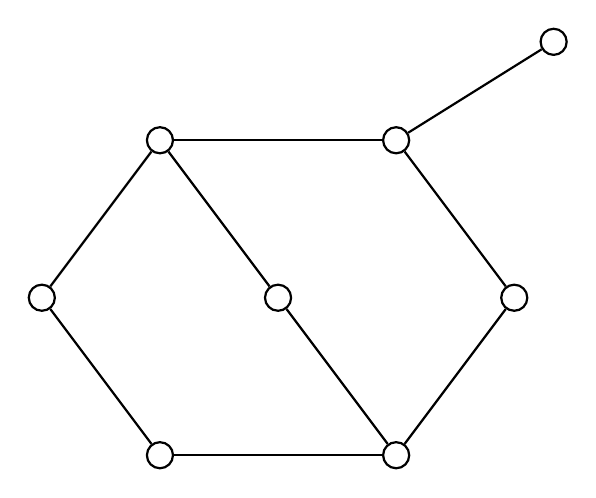
\begin{tikzpicture}
    [>=stealth,thick]
    %Nodes
    \node[circle,draw] (A) at (-4,2){};
    \node[circle,draw] (B) at (-1,2){};
    \node[circle,draw] (C) at (-2.5,4){};
    \node[circle,draw] (D) at (-2.5,0){};
    \node[circle,draw] (E) at (0.5,4){};
    \node[circle,draw] (F) at (2.5,5.25){};
    \node[circle,draw] (G) at (2,2){};
    \node[circle,draw] (H) at (0.5,0){};

    %Edges
    \draw[-] (A) -- (C) node []{};
    \draw[-] (A) -- (D) node []{};
    \draw[-] (C) -- (B) node []{};
    \draw[-] (B) -- (H) node []{};
    \draw[-] (D) -- (H) node []{};
    \draw[-] (H) -- (G) node []{};
    \draw[-] (C) -- (E) node []{};
    \draw[-] (E) -- (F) node []{};
    \draw[-] (E) -- (G) node []{};
    
\end{tikzpicture}

\end{document}